%%%%%%%%%%%%%%%%%%%%%%%%%%%%%% -*- Mode: Latex -*- %%%%%%%%%%%%%%%%%%%%%%%%%%%%
%% project.tex -- 
%% Author          : Philip Johnson
%% Created On      : Tue Nov  4 10:26:48 1997
%% Last Modified By: 
%% Last Modified On: Fri Jan 19 16:19:09 2007
%% RCS: $Id$
%%%%%%%%%%%%%%%%%%%%%%%%%%%%%%%%%%%%%%%%%%%%%%%%%%%%%%%%%%%%%%%%%%%%%%%%%%%%%%%
%%   Copyright (C) 1997 Philip Johnson
%%%%%%%%%%%%%%%%%%%%%%%%%%%%%%%%%%%%%%%%%%%%%%%%%%%%%%%%%%%%%%%%%%%%%%%%%%%%%%%
%% 

\section{Motivation}

The goal of the Science of Design (SoD) program is to bring creative,
scientific advances to the design of software artifacts and systems.  New
paradigms, concepts, approaches, models, and theories arising from this
program should improve the processes of constructing, evaluating, and
modifying software-intensive systems. Important research questions include
the design and evaluation of software architectures with respect to their
quality and understandability; design optimization in the presence of
contradictory, inconsistent, emergent, and/or ambiguous requirements; and
analysis of tradeoffs between information and software design.  In all
cases the program focus is on basic research to advance the science of
software-intensive design, and on the effective application of SoD research
outcomes to the design of practical software intensive systems and their
integration into educational curricula.

While the programmatic emphasis on ``creative'' approaches implies a
preference for revolutionary over evolutionary advances, and
interdisciplinary over single discipline approaches, the equal emphasis on
``scientific'' approaches implies that this creativity should be explored
within a methodological context that supports, for example: 
\begin{itemize}
\item an ability to characterize the internal and external validity of the findings
\item the ability to replicate the results 
\item operational definitions for design characteristics and outcomes
relevant to the research, such as ``quality'', ``complexity'',
``performance'', ``usability'', ``maintainability'', and so forth.
\item systematic measurement of qualitative and quantitative metrics.
\end{itemize}

A first-order positive impact of the Science of Design program would be the
discovery of novel design techniques with demonstrable advantages in their
initial observed context of use.  However, such impact would be multiplied
if at least some of the project findings were generated in a way that
support direct comparison, combination, and/or meta-analysis.  Such an
approach would facilitate a new set of ``second-order'' impacts, such as
``Does the combination of design technique A with design technique B have
an additive, multiplicative, or negative effect on software quality?''
Comparability also accelerates the process of discovering the context
variables associated with research results; given two domains and two
design techniques, comparability facilitates the 2x2 evaluation. (Need to
say this better.)

One way to facilitate direct comparison, combination, and meta-analysis is
through the use of a testbed.  One form of testbed is a common artifact.
For example, in the HDCS project, the Mars Rover software was developed as
a common testbed for assessing different dependability techniques
\cite{MarsRoverTestBed}. A second kind of testbed is an experimental
infrastructure for standardized definition, collection, and analysis of
empirical measures.  Both kinds of testbeds are useful, and indeed
complementary.

This proposal describes how the Hackystat Framework can be applied as an
effective experimental infrastructure testbed for the Science of Design
program.  The Hackystat Framework has been under development for five years
and has been used in a wide variety of contexts, including design
evaluation support in the context of Test Driven Development. The research
advances we propose for the Hackystat Framework to support the Science of
Design program are admittedly incremental in nature, and thus would seem to
violate at least one of the stated goals of the program.  We wish to argue
at the outset of this proposal that when evaluating testbed technology for
Science of Design, the goals of the program are better supported by
supporting a mature testbed technology with demonstrated capabilities,
leaving the novelty for the design innovations themselves.  

The basic idea of Hackystat is to attach ``sensors'' to development tools
which capture either ``process'' or ``product'' data.  By process data, we
mean developer behaviors that can be detected through their interaction
with a tool.  For example, by instrumenting an interactive development
environment, Hackystat can detect developer behaviors such as when code is
compiled, unit tests are invoked, and so forth.  Because Hackystat attaches
timestamps to these events, it can provide a record of the sequence of
behaviors that occur.  By product data, we mean information produced by the
invocation of analysis tools on a software artifact.  This can include size
or structural complexity metrics, the count and types of quality assurance
problems detected by tools like Checkstyle, PMD, FindBugs, and so forth.  It is 
also possible to manually collect qualitative data and represent it in Hackystat,
which would enable a researcher to ``annotate'' subject data, or allow developers
to provide logs of their activities, and so forth.

For Hackystat to be of use as a testbed for projects in the Science of
Design program, it must be adapted to collect the process and product data
of importance to the project under study.  In addition, the project must be
carried out in such a way that important data is actually amenable to
collection and analysis via Hackystat.  Some of the research to be
performed in this proposal includes dialogue with currently funded Science
of Design participants to articulate their testbed requirements and to
extend Hackystat to support them.  In the related work section, we will use
project descriptions from previous SoD awards to illustrate some of the
issues that might arise in this process.

A key contribution of Hackystat is its ability to instrument not only the
specific tools and techniques developed as part of the SoD project, but
also the other tools and processes in a development environment that must
be used to develop software.  For example, a given SoD project might focus
on a requirements monitoring tool, which is just one component of the
overall software development process. When evaluating this tool, it would
be useful to understand when and where it is applied during development,
and whether it results in changes to other artifacts created. Hackystat
currently supports over 30 sensors for a variety of programming languages
and tool frameworks.

The next section of this proposal explores the requirements for a Science
of Design testbed.  The following section introduces the Hackystat
Framework, including two examples of use as an empirical testbed.  We then
review research related to science of design testbeds.  We next present a
project plan, and how we intend to facilitate adoption of the Hackystat
Framework by SoD participants. We conclude with a discussion of how this
proposal fulfills the NSF Merit Review criteria.

Issue: how can we lower the cost of comparability?  Several SoD proposals
talk about use of design verification techniques and their ability to
improve correctness, lower cost, etc.  If we can provide data within a
common framework, we can compare their effectiveness.

Emergent categories: Design verification/validation/automation through
formal techniques; end-user programming; economic/value-based design

An important research issue for Hackystat is to figure out how to
incorporate value-based costing in a way that makes sense for other
projects.

For example, some projects are quite explicit about going beyond
traditional cost models that are code-centric (economic approaches, end
user approaches) while other projects seem to maintain a much more
traditional approach to cost (design verification, etc.)

Make up a new tool name: SoDeT

\section{Requirements for a SoD Testbed}
Some of the requirements for a Science of Design testbed include:
\begin{itemize}
\item comparable data
\item simplified replication
\item meta-analysis
\item cross-project comparison
\item process conformance
\item infrastructure leverage
\item benchmark design problems.
\item data types: process, product, runtime behavior, maintenance.
\end{itemize}


\section{Science of Design Projects}

To understand more fully how the TfSoD can facilitate the overall Science
of Design program, it is helpful to review information regarding previously
funded SoD projects and discuss possible uses of a testbed. 

In the project ``Monitoring in support of design science principles'',
Robinson proposes the use of a tool called ReqMon to provide guidance on
when and what aspects of software should be evolved by dynamically
monitoring individual user goals. The ReqMon Framework defines a language
for requirements and monitor definitions, plus monitoring tools to
instrument running systems for compliance with their requirements. By 
attaching sensors to both the ReqMon tool and other development tools, 
TfSoD can be used to simplify the ability of these researchers to generate
comparable data concerning: 
(a) the time spent defining and modifying requirements definitions;
(b) how that activity is interleaved with other development activities; and 
(c) how often the monitoring tools actually find a violation

In ``Teaching Creativity and Conceptual Representation, 
a Design Toolkit'', Amoussou proposes the creation of a new curriculum for
Science of Design, which includes  the creation of design artifacts.  If
sensors can be created for the tools that create these artifacts, then 
TfSoD can be used to better understand the way that the introduction of 
these new techniques change the way students generate designs, the level
of collaboration that takes place around design, and so forth. 

In ``Tools and Techniques for On-the-fly Design of Business
Process Integration'', Su proposes to develop a formal framework and
collection of tools that aid in the design (or re-design) and management of
business processes and business process integration. Su hypothesizes that
this targeted declarative framework can (a) increase precision and reduce
ambiguity in process specification, and (b) create flexibility though
support for incomplete specifications, leading to reduced development times
and higher quality code.  Use of TfSoD can provide the infrastructure required
to measure development time, and can facilitate evaluation of quality through 
use of automated quality assurance tools. By monitoring the use of other tools,
the testbed can also help reveal the way the declarative framework is integrated
into the overall development process.

In ``Design for Adaptivity and Reliable Operation of Software
Intensive Systems'', Abdelwahed proposes a semi-automated process based
upon mathematical models and control-theoretic techniques and supported by
tools for design, verification, and analysis. The intended outcome of this
research is to simplify the development of a large class of distributed
real-time and embedded software intensive systems.  TfSoD can provide 
infrastructure for instrumenting the design, verification, and analysis tools
produced through this research, along with the other tools (compilers, 
debuggers, run-time environments, etc.) required for development.  Such 
infrastructure can support understanding the time spent using the tools, 
the manner in which these design, analysis, and verification activities
are interleaved with other development activities, and the process impacts
of this approach. 

In ``Robust System Design Under Weak Component Assumptions'', Zhou proposes
a formal theory, language, and toolset for design and specification of
systems composed of imperfect components.  The language and toolset
supports analysis of a system's functional limits under different assumptions, 
and supports trade-off analysis between system assurance and component choice.
This research would appear to generate an operational definition of 
design ``quality'' in terms of a system's functional limits. A case study
using TfSoD instrumentation would reveal insights into the time spent
using the tool, and how developers interleave tool usage with other
development tasks (coding, compilation, debugging, etc.) 

In ``Comprehensibility as a Design Criterion'', Gamboa proposes to 
modify two program analysis tools (Daikon and AbsInt) for use as an 
empirical measure for design quality in terms of its ``comprehensibility''. 


\begin{figure*}[ht]
\small
\begin{tabular}{|p{0.70in}|p{1.85in}|p{1.85in}|p{1.85in}|} \hline
{\bf PI(s)} & {\bf Project Focus} & {\bf Tools Produced} & {\bf Outcome Measures/ \newline Hypotheses} \\ \hline

Abdelwahed &
Model-based real-time, \newline  embedded system design &
Model-based design, analysis, \newline verification tools  &
(Improved) design, \newline (Improved) implementation \\ \hline

Amoussou &
Design Education &
None indicated &
Curriculum toolkit, \newline Interdisciplinary education \\ \hline

Bailey &
Early stage UI design &
Visual sketching language, Tool support for early stage creative design &
Utility of language and tool, \newline Impact on creativity  \\ \hline


Basili, \newline Carver &
Architectural change management &
None indicated  &
Models of architectural change, faults, design \\ \hline

Batory &
Generative Programming &
None indicated &
Feature-based programs more amenable to synthesis, optimization, and evolution \\ \hline

Bodik &
Programming by sketching &
Sketching Synthesizer for Scientific Programs &
Automated implementation from high-level sketches \\ \hline

Boehm &
Value-based design &
Value-based software design tools &
Composable process patterns for value-based software design \\ \hline

Bultan &
Design for Verification &
None indicated &
Design patterns amenable to verification \\ \hline

Devanbu &
Open source design &
None indicated &
Impact of process on design  \\ \hline

Ernst &
Software design and testing &
Test generation from designs &
(Improved) execution, \newline (Improved) coverage \\ \hline

Findler \newline Felleisen &
Software markets, quality assurance, and design &
None &
Better understanding of how market mechanisms influence design \\ \hline

Fischer &
Participative software design &
Meta-design framework &
(Improved) participation in design, \newline (Continuous) design throughout software lifecycle \\ \hline

Flanagan &
Ethics and politics in design &
Values-in-design toolkit &
Best practices, handbook \\ \hline

Flatt, \newline Shivers &
Language ``towers'' &
Meta-tools for language notation design &
(More efficient) language design \\ \hline

Gamboa &
Design comprehensibility &
Enhanced Daikon, \newline Enhanced AbsInt &
Design quality (comprehensibility) \\ \hline


\end{tabular} 
\caption{Preliminary feasibility analysis of SoD Projects for SoDeT (1)}
\label{fig:sod}
\normalsize
\end{figure*}

\begin{figure*}[ht]
\small
\begin{tabular}{|p{0.70in}|p{1.85in}|p{1.85in}|p{1.85in}|} \hline
{\bf PI(s)} & {\bf Project Focus} & {\bf Tools Produced} & {\bf Outcome Measures/ \newline Hypotheses} \\ \hline

Getoor &
Design processes for semantic data integration, transformation, and sharing &
Data viewers, mappers, transformation languages &
Benchmark for schema and mapping discovery \\ \hline

Goel &
Teleological Reasoning in Design &
Interactive software design environment &
Case study data, data on efficacy of teleological-based design  \\ \hline

Guzdial &
End-user programming &
None indicated &
Design knowledge of end-user programmers \\ \hline

Hicks &
Software Design Evaluation &
Tools for software design evaluation &
Benchmark programs for software design evaluation \\ \hline

Jackson \newline Perry &
``Prescriptive'' software architecture descriptions &
Alloy constraint system \newline Compositional Compiler  &
(Improved) design quality \newline (Improved) understanding of design trade-offs \\ \hline

Jagadish &
Incremental design of XML information systems &
Automated mapping/translation of schema &
(Reduced) effort to design and maintain information stores \\ \hline

Klein &
Non-linear negotiation for design &
Taxonomic knowledge base of designs &
(Improved) component selections, \newline (Improved) design efficiency \\ \hline

Liu \newline Stoller &
Reconciling modularity and efficiency &
Language for design knowledge &
Design invariants \\ \hline

Lorenz \newline Attie &
Design locality &
``Pairwise composition'' analysis and verification tools &
Modular, modifiable, and maintainable designs \\ \hline

Mok \newline Abdelzaher &
Embedded software design &
Feedback control and stability tools &
(Improved) reliability \newline (Reduced) cost \\ \hline

Paul &
Multiprocessor chip design &
None indicated. &
``Characterize-and-invent'' chip design paradigm \\ \hline

Rajlich &
Design of incremental change &
Static program analysis &
(Improved) software quality \newline (Reduced) software maintenance costs \\ \hline


\end{tabular} 
\caption{Preliminary feasibility analysis of SoD Projects for SoDeT (2)}
\label{fig:sod}
\normalsize
\end{figure*}

\begin{figure*}[ht]
\small
\begin{tabular}{|p{0.70in}|p{1.85in}|p{1.85in}|p{1.85in}|} \hline
{\bf PI(s)} & {\bf Project Focus} & {\bf Tools Produced} & {\bf Outcome Measures/ \newline Hypotheses} \\ \hline

Reiss &
Semantic component design &
None indicated &
More controllable software design \\ \hline

Robinson &
Requirements Monitoring, \newline End-user goals &
Run-time compliance monitor &
End-user requirements, \newline Requirements changes \\ \hline

Roth &
Learning based programming &
Incorporation of machine-learning into programming language &
(Better) programming abstractions \\ \hline


Shaw &
Managing uncertainty in design &
None indicated &
Requirement uncertainty representations, \newline Reducing user uncertainty \\ \hline

Sheard &
Semantics-based system design &
Omega &
Integrated specification, implementation, design  \\ \hline

Shipman &
Design by end-user &
End-user design ``construction kit'' \newline Design Repository &
(Improved) stakeholder communication, involvement in design \\ \hline

Sreenivas &
Design of discrete event system supervisory policies &
None indicated &
(Improved) discrete event system designs \\ \hline

Siskind &
Functional programming &
None indicated &
Framework for differentiation of functions through symbolic manipulation \\ \hline


Su &
Business Process Specification &
Business Process Design, \newline Business Process Management &
(Reduced) development time, \newline (Improved) code quality \\ \hline

Sullivan \newline Griswold &
Economic analysis of design &
None indicated &
Economic ``value'' of designs \\ \hline

Taha &
Synthesizing device drivers &
MetaOCaml &
(Improved) design process \\ \hline

Tanimoto &
Collaborative Design &
Collaborative design communication, evaluation, \newline T-Star &
End-user design, \newline Visualized design spaces \\ \hline

Taylor &
Architectural Design &
Tools for applying ``proven'' architectural styles &
Principles, practices, tools for architectural design \\ \hline


Vardi &
Automated design &
Assertion based automated design tool &
(Higher) quality, \newline (Shorter) design cycles \\ \hline

Xie &
Feedback-based architectures &
Tools for mission-critical software &
(Improved) reliability, \newline (Reduced) cost \\ \hline

Zhou &
Design and specification with imperfect components &
Model-based analyzer, verifier &
Functional limits of feasible systems \\ \hline




\end{tabular} 
\caption{Preliminary feasibility analysis of SoD Projects for SoDeT (3)}
\label{fig:sod2}
\normalsize
\end{figure*}




Things to think about:

- There are tools to support the development of designs

- There are (hopefully) mechanisms to support evaluation of designs

- Big questions: what are the process impacts of these tools; for example, 
do they change the way other aspects of development (coding, testing, 
maintenance) are performed?   Are the amenable to Agile or Plan-based 
development? 


- Some people equate ``scientific'' with formality--i.e.  the ability to
prove properties of a system.  I look at ``scientific'' as a method---a way
to derive evidence and interpret it.



\section{Hackystat}

For the past five years, we have been developing a framework for
automated software development process and product metric collection and
analysis called Hackystat.  This framework differs from other approaches to
software product and process measurement in one or more of the following ways:

\begin{itemize}

\item Hackystat uses sensors to unobtrusively collect data from development
environment tools; there is no chronic overhead on developers to collect
product and process data.  In contrast, tools such as the Process Dashboard
\cite{PSPDashboard} involve manual data collection. 

\item Hackystat is tool, environment, process, and application agnostic.
The architecture does not suppose a specific operating system platform, a
specific integrated development environment, a specific software process,
or specific application area.  A Hackystat system is configured from a set
of modules that determine what tools are supported, what data is collected,
and what analyses are run on this data. In contrast, tools such as TSP Tool
\cite{TSPTool} implement support for a fixed set of metrics under a fixed
process on a single platform.

\item Hackystat is intended to provide in-process project management
support. Traditional software metrics approaches, such as 
the NASA Metrics Data Program \cite{MDPRepository},  are based upon the
``project repository" method, in which data from prior completed projects
are used to make predictions about a future
project. In contrast, Hackystat is designed to continuously collect data from a current,
ongoing project, and use that data as feedback into the current project.

\item Hackystat is open source and is available to the academic and
commercial software development community for no charge. In contrast,
commercial toolkits such as MetricCenter \cite{MetricCenter} are closed
source and require licensing fees.

\end{itemize}

The design of Hackystat \cite{csdl2-02-07} reflects prior 
research in our lab on software measurement, beginning with research into
data quality problems with the PSP \cite{csdl-98-11} and continuing with
research on the LEAP system for lightweight, empirical, anti-measurement
dysfunction, and portable software measurement \cite{csdl2-00-03}.

\begin{figure*}[ht]
  \centering
  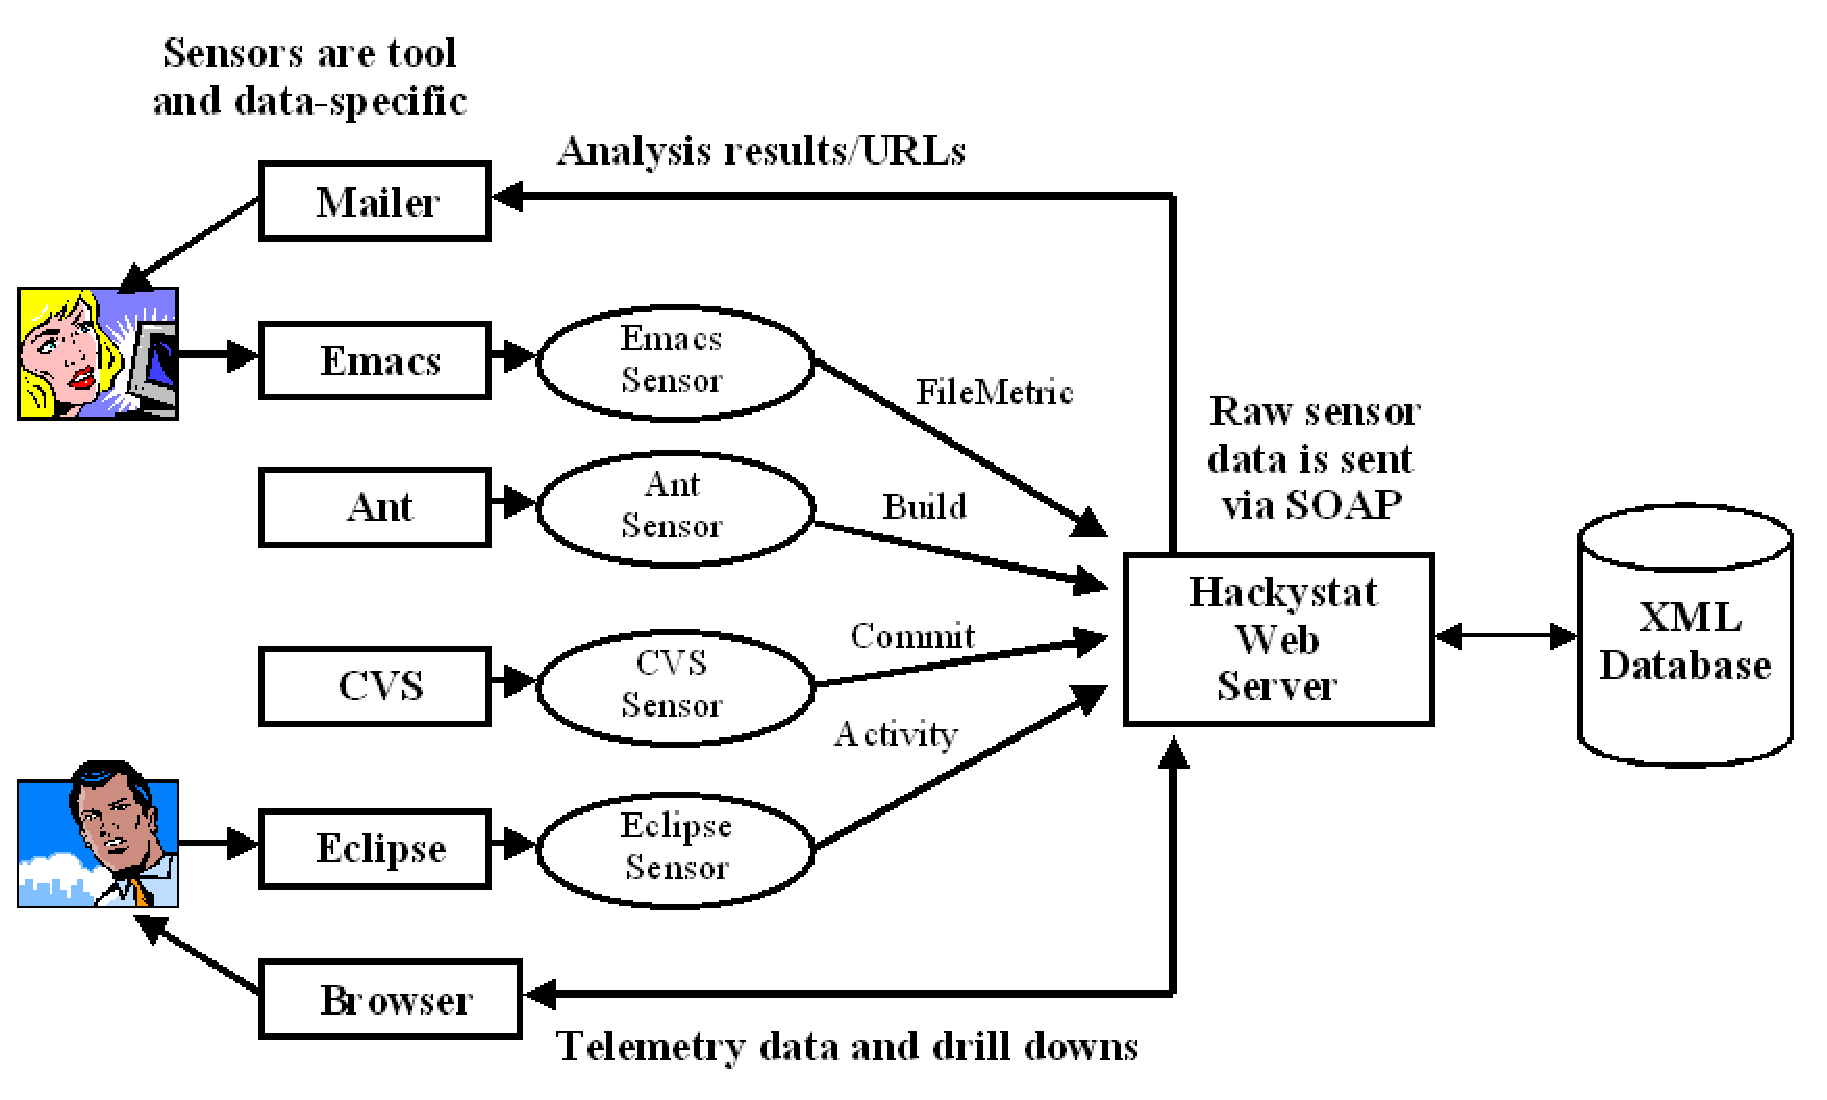
\includegraphics[width=0.60\textwidth]{architecture.eps}
  \caption{The basic architecture of Hackystat.}
  \label{fig:architecture}
\end{figure*}

To use Hackystat, the project development environment is instrumented by
installing Hackystat sensors, which developers attach to the various tools
such as their editor, build system, configuration management system, and so
forth. Once installed, the Hackystat sensors unobtrusively monitor
development activities and send process and product data to a centralized
web server.  If a user is working offline, sensor data is written to a
local log file to be sent when connectivity can be re-established.  Project
members can log in to the web server to see the collected raw data and run
analyses that integrate and abstract the raw sensor data streams into
telemetry.  Hackystat also allows project members to configure ``alerts``
that watch for specific conditions in the sensor data stream and send email
when these conditions occur. Figure \ref{fig:architecture} illustrates the
basic architecture of the system.

Hackystat is an open source project. Its sources, binaries, and
documentation are freely available online.  We also maintain a public
server running the latest release of the system at
http://hackystat.ics.hawaii.edu.  Hackystat has been under active
development for approximately five years, and currently consists of
approximately 2500 classes and 300,000 lines of code.  Sensors are available
for a variety of tools including Eclipse, Emacs, JBuilder, Jupiter, Jira,
Visual Studio, Ant, JUnit, JBlanket, CCCC, DependencyFinder, Harvest, LOCC,
Office, CVS, and SVN.

Hackystat is being used in a variety of academic and industrial contexts.
At the University of Hawaii, Hackystat has been  integrated into the
undergraduate and graduate software engineering curriculum, and is
used by approximately 50 students per year to support project
development \cite{csdl2-03-12}.  A researcher from the Free University of
Bozen came to Hawaii to study the Hackystat system in support their research on
PROM \cite{Sillitti03}.  Researchers at the University of Maryland are
using Hackystat to support assessment of programmer effort
\cite{Hochstein05}.  Hackystat has been used at NASA's Jet Propulsion
Lab to analyze the daily build process for the Mission Data System
\cite{csdl2-03-07}.  Finally, Hackystat is being used at SUN Microsystems
to support research on high performance computing system development
productivity \cite{csdl2-04-03}.


\section{Related work}

- other metrics systems
- design evaluation literature


From: Peffers, et al (The Design Science Research Process)
5. Evaluation. Observe and measure how well the artifact supports a solution to the
problem. This activity involves comparing the objectives of a solution to actual observed
results from use of the artifact in the demonstration. It requires knowledge of
relevant metrics and analysis techniques. Depending on the nature of the problem
venue and the artifact, evaluation could include such items as a comparison of the artifact�s
functionality with the solution objectives from activity 2 above, objective
quantitative performance measures, such as budgets or items produced satisfaction
surveys, client feedback, or simulations. At the end of this activity the researchers can
decide whether to iterate back to step 3 to try to improve the effectiveness of the artifact
or to continue on to communication and leave further improvement to subsequent
projects. The nature of the research venue may dictate whether such iteration is feasible
or not.

Google: Science of Design Baldwin

From: Dreyfus.

Design science is a research paradigm in which designers (builders of systems) and
social scientists develop insights and knowledge through interaction with artifacts. The
artifact is an occasion for both independent and joint learning. Social scientists and
scientists of design provide descriptive knowledge of the nature of social and socialtechnical
interactions. Designers of systems incorporate this knowledge as they build new
systems and develop new insights into the process of designing and building systems.
During the process of evaluating the resulting artifact, new insights and knowledge are
developed by both social scientists and designers of systems.

Chen Value Driven paper is an SoD project.

Mikael Lindvall, Ioana Rus, Paolo Donzelli, Atif Memon, Marvin Zelkowitz, Aysu Betin-Can, Tevfik Bultan, Chris Ackermann, Bettina Anders, Sima Asgari, Victor Basili, J�rg Fellmann, Daniel Hirschbach, Lorin Hochstein, Forrest Shull, Roseanne Tvedt and Daniel Pech. ``Experimenting with Software Testbeds for Evaluating New Technologies.'' To appear in Empirical Software Engineering.
ps   pdf

evidence-based research
\section{project structure}
- Webinar: introduce system
- solicit requirements from SoD community
  - sensors
  - analyses
- create common/competing operational definitions
- public repository and/or private servers
- facilitate training, support,
- privacy issues.

\section{Merit Review Criteria}


-intellectual merti
-broader impacts

- integration of research and education
- integrating diversity
- The Program is looking for new and creative ways of thinking about a Science of Design discipline for software-intensive systems. Incremental research will not be funded. Project Descriptions must present a vision for a Science of Design that forms the context for the contributions of the proposal.




